\section{METODOLOGÍA}
\subsection{Obtención de datos}
Para poder entrenar un red neuronal capaz de predecir el resultado de un test tipo MOS realizado sobre un sistema de texto a voz, se necesita generar una base de datos con los resultados de un gran numero de algoritmos de síntesis vocal, acompañados de una etiqueta que represente su puntuación final obtenida de una prueba MOS. También se puede incluir en esa base de datos, ejemplos de voces humanas reales, y señales de voz sintetizadas, procesadas digitalmente.

Con el objetivo de generar esta robusta base de datos, en primera instancia se recolectaron ejemplos de un gran numero de sistemas de generación de voz humana disponibles. Los ejemplos a sintetizar fueron tomados de la lista de frases que forman parte del cuerpo de la base de datos de openSLR \cite{opensrl}: una base de datos generada por un equipo de investigación de Google, con el fin de entrenar sistemas de TTS y de ASR para idiomas de bajos recursos. Las lista completa de frases utilizadas son incluidas en el Anexo I.

En la Tabla \eqref{tab:dataset} se detallan los sistemas de texto a voz utilizados en la generación de la base de datos. Todos los ejemplos fueron sintetizados en castellano. El código de región exhibido en la tabla esta basado en el estándar ISO 639-1 para determinar la región de la voz sintetizada.

La base de datos incluye distintas voces sintetizadas con servicios profesionales de síntesis como Amazon Polly, Microsoft Azure, Speechello y Neurasound, sistemas concatenativos como Loquendo y la implementación TTS de Thomas Dewitte, servicios experimentales basados en Fastpich, y voces humanas reales pertenecientes al banco de voces OpenSRL.


\begin{table}[H]
\centering
\caption{Composición de la base de datos generada. Código de región de acuerdo a ISO 639-1.}
\label{tab:dataset}
\begin{tabular}{@{}ccccc@{}}
\hline
                                                                        & \textbf{Descripción}                                                          & \textbf{Región}                                                          & \textbf{Cant. de voces} \\ \hline
\textbf{\begin{tabular}[c]{@{}c@{}}Amazon \\ Polly\end{tabular}}        & Implementación privada                                                        & \begin{tabular}[c]{@{}c@{}}es-us/es-mx\\ /es\end{tabular}                & 8                       \\ \hline
\textbf{\begin{tabular}[c]{@{}c@{}}Microsoft \\ Azure\end{tabular}}     & Implementación privada                                                        & \begin{tabular}[c]{@{}c@{}}es-ar/es-bo\\ /es/es-mx\end{tabular}          & 8                       \\ \hline
                                                                        & Implementación privada (I.A.)                                                 & es-us/es-mx                                                              & 2                       \\
\multirow{-2}{*}{\textbf{Speechello}}                                   & Implementación privada                                                        & \begin{tabular}[c]{@{}c@{}}es-us/es-mx\\ /es\end{tabular}                & 5                       \\ \hline
\textbf{Neurasound}                                                     & Implementación privada                                                        & \begin{tabular}[c]{@{}c@{}}es-ar/es-cl/es-bo/\\ es-pe/es-pr\end{tabular} & 14                      \\ \hline
\textbf{Loquendo}                                & Sistema concatenativo                                                         & es                                                                       & 1                       \\ \hline
\textbf{\begin{tabular}[c]{@{}c@{}}text-to-\\ speech\end{tabular}}      & Librería de Python                                                            & es                                                                       & 1                       \\ \hline
\textbf{\begin{tabular}[c]{@{}c@{}}Fastpitch - \\ HiFiGan\end{tabular}} & \begin{tabular}[c]{@{}c@{}}Implementación con \\ transformadores\end{tabular} & es-ar                                                                    & 4                       \\ \hline
\textbf{DC-TTS}                                                         & Red convolucional                                                             & es-ar                                                                    & 7                       \\ \hline
\multicolumn{1}{l}{\textbf{TacoTron2}}                                  & Modelo secuencial                                                             & es                                                                       & 1                       \\ \hline
\textbf{OpenSRL}                                                        & Grabaciones de personas                                                       & es-ar                                                                    & 48                      \\ \hline
\end{tabular}
\end{table}

Esta base de datos inicial fue limpiada, transformada  y reducida durante el diseño de la prueba subjetiva, como será expuesto en la sección 4.3.


\subsection{Expansión artificial de datos}

Con el objetivo de variar los tipos de voces obtenidos en la sección previa, se llevo a cabo un proceso de expansión artificial de datos basada en distintas técnicas de procesamiento digital. Las mismas son detalladas a continuación:
\begin{itemize}
    \item \textbf{Alteración de largo tracto vocal (VTLP)}: 300 ejemplos de voces sintetizadas fueron procesados por este algroritmo, la implementación utilizada y el factor de deformación de VTLP (elegido aleatoriamente entre 0,9 y 1,1 para cada ejemplo) se basaron en recomendaciones detalladas por Jaitly et al. \cite{vtlp}.
            
    \item Alteración de fase (Algoritmo de Griffin-Lim): 500 ejemplos de voces reales y 100 ejemplos de voces sintetizadas fueron procesadas por este algoritmo de acuerdo al procedimiento especificado en la sección 2.3.2. 
    
\end{itemize}{}

\subsection{Diseño de la prueba subjetiva}

El diseño de la prueba subjetiva se basa en las especificaciones provistas por las recomendaciones del estándar ITU-T Rec. P.807. Todos los sujetos encuestados cumplieron con la condición de ser normo-oyentes.

El test consiste en la evaluación subjetiva de una serie de audios cortos que contienen distintas voces (2 a 6 segundos de duración). La duración total del test es de aproximadamente 8 minutos. Los ejemplo deben ser evaluados en una escala de tipo Likert de 5 puntos. La cantidad máxima de audios que un sujeto puede evaluar es de 50. El propósito de la encuesta subjetiva es el de etiquetar los audios recolectados previamente, con una puntuación. La cantidad de etiquetas necesarias está determinadas por el entrenamiento de la red neuronal que se desarrollará a posteriori. Un precedente útil se puede tomar del trabajo de Deja et al.[13] en el cual se llevó a cabo una metodología similar. Sujeto a la cantidad de audios que evalúe cada persona, en principio son necesarios alrededor de 100 sujetos de prueba, asumiendo que cada sujeto de prueba evalúe alrededor de 50 audios.

Una síntesis de las instrucciones presentadas a los participantes de la encuesta es provista a continuación:

\large{\textbf{Instrucciones}}

\normalsize

A continuación vas a escuchar una serie de distintos tipos de voces generados por computadoras. El propósito de este test es evaluar la calidad de cada archivo, para poder subsecuentemente utilizar esa información en un sistema de evaluación automático de voces sintetizadas.

Para cada ejemplo se deberá proveer una calificación de acuerdo a la siguiente escala. (Escala MOS para la naturalidad de una voz, Tabla \eqref{tab:instrucciones})

\begin{table}[H]
\centering
\caption{Escala MOS para la naturalidad de una voz}
\label{tab:instrucciones}
\begin{tabular}{cccll}
\textbf{Puntaje} & \textbf{Calidad del habla} & \textbf{Naturalidad}                    &  &  \\ \cline{1-3}
5                & Excelente                  & Completamente natural                   &  &  \\
4                & Buena                      & Bastante natural                        &  &  \\
3                & Aceptable                  & Natural y antinatural en partes iguales &  &  \\
2                & Mediocre                   & Bastante antinatural                    &  &  \\
1                & Mala                       & Completamente antinatural               &  & 
\end{tabular}
\end{table}

Los siguientes ejemplos ilustran el significado de cada puntaje. Sin embargo para realizar la prueba es importante tener en cuenta que se escucharan otros tipos de voces muy distintas, con distorsiones o artefactos no presentes previamente. Por lo tanto, estos ejemplos no cubren la totalidad de las posibilidades  que pueden esperar escuchar.

\large{\textbf{Ejemplos}}

\normalsize

El siguiente ejemplo presenta una voz humana y tiene un puntaje de referencia de 5.0

\begin{figure}[H]
    \centering
    
\includegraphics[scale=0.02]{imagenes/ale.jpg}
\end{figure}

El siguiente ejemplo presenta una voz sintetizada, puntaje de referencia de 4.0

\begin{figure}[H]
    \centering
    
\includegraphics[scale=0.02]{imagenes/ale.jpg}
\end{figure}

El siguiente ejemplo presenta una voz sintetizada, puntaje de referencia de 3.0

\begin{figure}[H]
    \centering
    
\includegraphics[scale=0.02]{imagenes/ale.jpg}
\end{figure}

El siguiente ejemplo presenta una voz sintetizada, puntaje de referencia de 2.0

\begin{figure}[H]
    \centering
    
\includegraphics[scale=0.02]{imagenes/ale.jpg}
\end{figure}

El siguiente ejemplo presenta una voz sintetizada, puntaje de referencia de 1.0

\begin{figure}[H]
    \centering
    
\includegraphics[scale=0.02]{imagenes/ale.jpg}
\end{figure}

Tener en cuenta que la calidad de los ejemplos que deberán clasificar puede ser distinta a la escuchada en estos ejemplos.


\subsubsection{Selección de respuestas validas}
Con el fin de descartar respuestas atípicas, se toman ciertos criterios para considerar validos los resultados de una prueba subjetiva:
\begin{itemize}
    \item Para cada ejemplo que se debe calificar, se tiene previamente un valor estimativo de la calidad esperada, extraído de encuestas previas y análisis objetivos. Por lo tanto si un candidato responde azarosamente, o simplemente deriva un criterio de calificación incorrecto por falta de claridad en las instrucciones,  es posible identificar y descartar sus respuestas.
    \item Se mide el tiempo de respuesta de cada estimulo. Se descartan los resultados que hayan sido entregados en un tiempo menor a un cierto umbral.
    \item Se toma los ejemplos a calificar de voces humanas reales como un “ancla", símil al concepto presente en otros tests subjetivos como el MuSHRA.
\end{itemize}

\subsubsection{Redistribución de audios a clasificar}

Para prevenir el sesgo de “ecualización de rango", los ejemplos provistos a los sujetos de prueba deben seguir una distribución uniforme respecto del rango de calidad total MOS definido para la naturalidad de la voz. La distribución de la base de datos debe ser perpetuamente balanceada en la medida que se obtienen resultados de distintas encuestas para asegurar la minimización de este sesgo.

Se llevó a cabo una prueba piloto de la evaluación propuesta que involucro a 5 participantes que calificaron 50 audios cada uno. Con los resultados obtenidos, se determinó un leve desbalanceo en en la calidad de los ejemplos sintetizados. En base a esto, se redefinió la base de datos obtenida previamente, para incluir más ejemplos de calidad estimada en el rango de 4,0 a 5,0. 


\subsection{Sistema de predicción de MOS}

\subsubsection{Funcionamiento general}
El funcionamiento del modelo de predicción cuenta de 3 etapas fundamentales: 1) Extractor de espectrograma de Mel y segmentación, 2) Extracción de características acústicas por franja, y 3) Extracción de características temporales. En la Figura \eqref{fig:fgeneral} se presenta un diagrama de la arquitectura implementada, que consiste de una modificación del modelo propuesto en \cite{qualityEst}.

\begin{figure}[h]
    \centering
    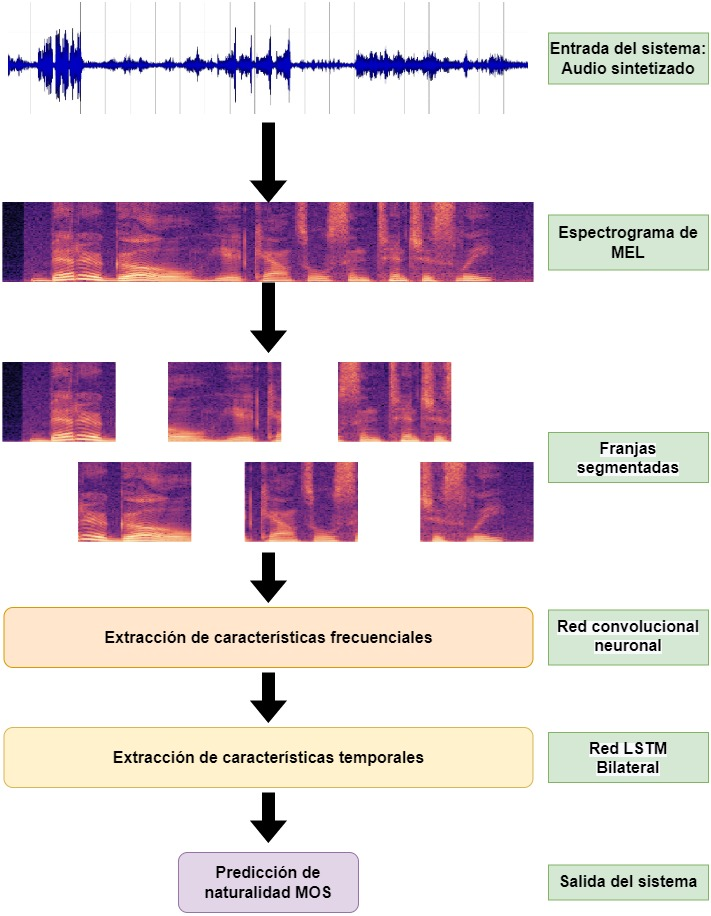
\includegraphics[scale=.45]{imagenes/funcionamiento_general.jpg}
    \caption{ Funcionamiento general del modelo de predicción de naturalidad MOS.}
    \label{fig:fgeneral}
\end{figure}

En primer lugar se extraen espectrogramas de Mel del audio a evaluar, separados en distintos segmentos con un cierto grado de solapamiento. Luego dichos segmentos son tomados como entrada de una red neuronal convolucional que extrae características útiles para predecir calidad sonora. Estas características se entregan a una red bilateral de larga-corta duración (BLSTM) que modela las dependencias temporales propias del discurso humano. La ultima capa completamente conectada de este segmento del modelo tiene como salida la predicción de naturalidad MOS.

\subsubsection{Segmentación en espectrogramas de MEL}
La entrada de la red neuronal convolucional toma espectrogramas de Mel generados a partir de una FFT con un tamaño de ventana de 20 ms y salto de 10 ms. El ancho de cada segmento es de 15, lo que equivale a 150 ms, y la altura es de 48 (48 x 15). La frecuencia máxima de análisis es de 20 kHz (muchos de los audios en el dataset tienen frecuencias de muestreo distintas). El tamaño de salto entre cada segmento es de 4 (40 ms), dando un cierto solapamiento de segmento a segmento. 

\subsubsection{Red CNN-BiLSTM}
Esta sección del modelo esta basado en la red siamés propuesta en \cite{qualityEst}. En la Figura \eqref{fig:cnn} se ofrece un diagrama para representar las distintas capas de este segmento del algoritmo de predicción. 

\begin{figure}[h]
    \centering
    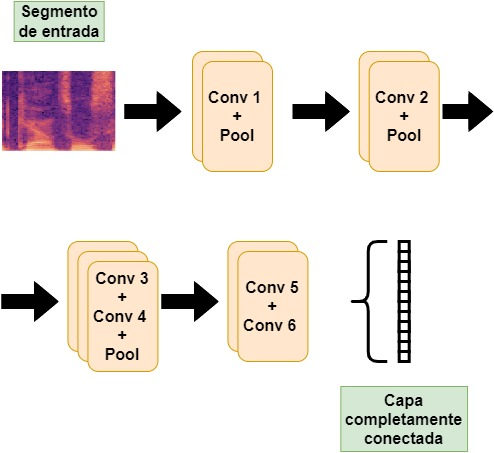
\includegraphics[scale=.45]{imagenes/cnn.jpg}
    \caption{ Arquitectura de la red neuronal convolucional. Cada capa esta acompañada por una activación de tipo ReLU.}
    \label{fig:cnn}
\end{figure}




La red esta tiene 6 capas convolucionales concatenadas, formadas por filtros de distintos tamaños como se puede observar en la Tabla \ref{tab:cnn}, donde N se corresponde con el numero de segmentos extraídos en la etapa previa, que depende de la duración del audio analizado. La salida de cada capa atraviesa una activación de tipo ReLU.

\begin{table}[]
\centering
\caption{Arquitectura de la red neuronal convolucional}
\label{tab:cnn}
\begin{tabular}{lllll}
\textbf{Capa}      & \textbf{Dimensión} &  &  &  \\ \cline{1-2}
Entrada            & Nx1x48x15          &  &  &  \\ \cline{1-2}
Conv1              & Nx16x48x15         &  &  &  \\
Pool               & Nx16x24x8          &  &  &  \\ \cline{1-2}
Conv2              & Nx32x24x8          &  &  &  \\
Pool-Perdida(20\%)  & Nx32x12x4          &  &  &  \\ \cline{1-2}
Conv3              & Nx64x12x4          &  &  &  \\
Conv4              & Nx64x12x4          &  &  &  \\
Pool-Perdida(20\%)  & Nx64x6x2           &  &  &  \\ \cline{1-2}
Conv5-Perdida(20\%) & Nx64x6x2           &  &  &  \\
Conv6              & Nx64x6x2           &  &  &  \\ \cline{1-2}
FC                 & Nx20               &  &  & 
\end{tabular}
\end{table}

La salida de esta etapa es utilizada como la entrada de una red de larga-corta duración bidireccional, de 1 sola capa con 128 unidades escondidas que se encarga de modelar las dependencias temporales de la señal y estimar finalmente la naturalidad del habla.

\subsubsection{Entrenamiento y detalle de la implementación}
El entrenamiento partió de pesos pre-entrenados con el NISQA Corpus \cite{nisqacorpus} una base de datos de audios en ingles evaluados subjetivamente por un gran numero de participantes. El ajuste fino de la red final se realizo sobre ese modelo, dividendo los resultados obtenidos de la encuesta subjetiva realizada en 80\% para el entrenamiento, y 20\% para la validación. 

El código necesario se implemento en el lenguaje de programación Python, sobre la biblioteca de DNN PyTorch y se encuentra disponible de en linea, en un repositorio \cite{repogit}. La velocidad de aprendizaje fue fijada en 0,001, se utilizo el optimizador Adam y se eligió la función de perdida consiente de sesgos, basándose en la metodología propuesta por \cite{biasloss}.

\subsection{Evaluación objetiva del sistema propuesto}

Para refinar el funcionamiento del modelo propuesto, (configuración de hiperparametros y características de la red propuesta), se analizan 2 métricas objetivas: correlación cruzada de Pearson ρ (PCC) y el error cuadrático medio (RMSE). {\color{red} \textit{En base a estas métricas se definirá el modelo final.}} \color{black} 

Para comparar el modelo propuesto con otras redes de predicción de calidad, ambas métricas propuestas son contrastadas con distintas soluciones del estado del arte: NISQA V1, NISQA V2 y ANIQUE+. La comparación se realiza sobre un subconjunto de ejemplos tomados de la base de datos desarrollada y evaluada subjetivamente a lo largo de este trabajo. Se evalúa el RSME y el PCC promedio sobre la totalidad del conjunto de audios, y también en distintas categorías como se presenta en la sección 5. 

En total, para cada modelo predictivo se evaluaron 200 audios, comparando el pronostico obtenido con el resultado subjetivo obtenido previamente. Se calcula RSME y PCC por estimulo, y seguidamente se obtiene un promedio de ambas métricas a nivel de cada sistema evaluado.


\newpage